\documentclass[runningheads]{svproc}

\usepackage{graphicx}
\usepackage{amsmath}
\usepackage{hyperref}
\usepackage{booktabs}
\usepackage{multirow}
\usepackage{xcolor}

\begin{document}

\mainmatter

\title{Explainable AI for Seismic Signal Classification: A 1D CNN Approach with Integrated Gradients}

\author{Addel Vidal García \and Alejandro Colón Álvarez \and Miguel Ángel Banteurt Blanco}

\institute{
Facultad de Ingeniería Informática, Universidad de las Ciencias Informáticas, La Habana, Cuba \\
\email{\{avidal, acolon, mbanteurt\}@uci.cu}
}

\maketitle

\begin{abstract}
The automatic classification of seismic signals is a critical task in modern seismology, with direct applications in early warning systems and seismic monitoring. Deep learning models, particularly Convolutional Neural Networks (CNNs), have demonstrated high performance in this domain. However, their black-box nature limits trust and adoption in safety-critical scenarios. This paper presents a 1D CNN architecture for classifying seismic signals into noise and seismic event categories, combined with the Integrated Gradients method from Explainable AI (XAI) to interpret model decisions. We evaluate the model on both synthetic data, generated through a computational model based on damped sinusoidal envelopes, and real data acquired from the global FDSN network (station IU.ANMO). Results show 100\% accuracy on synthetic data and 87.5\% on real data, demonstrating the feasibility of the approach while highlighting the importance of XAI for understanding model behavior in realistic conditions. The complete implementation is publicly available to ensure reproducibility.

\keywords{Explainable AI \and Integrated Gradients \and 1D CNN \and Seismic Signal Classification \and XAI \and Deep Learning}
\end{abstract}

\section{Introduction}

The detection and classification of seismic signals is a fundamental task in seismology, with applications ranging from early warning systems to the characterization of fault structures \cite{mousavi2019stead}. Traditional methods rely on manual feature extraction and threshold-based detection, which are labor-intensive and prone to errors in noisy environments.

In recent years, deep learning approaches, particularly Convolutional Neural Networks (CNNs), have shown remarkable performance in seismic signal classification \cite{ieee2024cnn, ieee2025seismic}. However, the lack of interpretability in these models remains a significant barrier to their adoption in operational seismological services. Explainable AI (XAI) methods address this limitation by providing insights into the decision-making process of neural networks \cite{sundararajan2017axiomatic}.

This work presents a complete pipeline for seismic signal classification using a 1D CNN, combined with Integrated Gradients for model interpretability. The main contributions are:

\begin{itemize}
\item Implementation of a 1D CNN architecture specifically designed for raw seismic waveform classification.
\item Generation of synthetic seismic data based on a physically-inspired computational model.
\item Application of Integrated Gradients to explain model predictions on both synthetic and real data.
\item Evaluation on real seismic data from the global FDSN network.
\item Public release of the complete implementation for reproducibility.
\end{itemize}

\section{Related Work}

The application of CNNs to seismic signal processing has been extensively studied. Mousavi et al. \cite{mousavi2019stead} introduced the STanford EArthquake Dataset (STEAD), establishing a benchmark for AI-based seismic detection. Recent works have explored 1D CNN architectures for direct waveform analysis \cite{ieee2024cnn, repository2024ncsu}, demonstrating competitive performance with traditional methods.

Data augmentation techniques have proven essential for improving CNN performance on seismic data \cite{science2025augmentation}. The combination of CNN with LSTM networks has also been explored for time-windowed earthquake detection \cite{journal2024cnnlstm}.

In the XAI domain, Sundararajan et al. \cite{sundararajan2017axiomatic} proposed Integrated Gradients, a method that satisfies important axioms for attribution methods. This technique has been successfully applied to time-series data, making it suitable for seismic signal analysis.

\section{Methodology}

\subsection{Synthetic Data Generation}

Synthetic data was generated to validate the pipeline before applying it to real data. The computational model is based on damped sinusoidal components that simulate the basic characteristics of seismic waves:

\begin{equation}
x(t) = A(t) \left[ \sin(2\pi f_1 t) + \alpha \sin(2\pi f_2 t) \right] + \epsilon(t)
\end{equation}

where $A(t) = A_0 e^{-\beta t}$ is a temporal envelope simulating amplitude decay, $f_1 = 5$ Hz and $f_2 = 9$ Hz represent dominant frequencies typical of local seismic events, $\alpha = 0.5$ is a weighting factor, and $\epsilon(t) \sim \mathcal{N}(0, 0.25)$ represents background noise.

A total of 1,000 signals were generated (500 noise, 500 synthetic events), each with 500 samples at 100 Hz sampling rate (5 seconds duration). Each signal was individually normalized to the range $[-1, 1]$.

\subsection{Real Data Acquisition}

Real seismic data was acquired from the global FDSN (Federated Digital Seismograph Networks) infrastructure, specifically from station IU.ANMO (Albuquerque, New Mexico), one of the most stable broadband stations worldwide, with continuous records since 1989.

The acquisition process involved:
\begin{enumerate}
\item Querying the USGS earthquake catalog for events with magnitude $M > 5.0$ between 2022 and 2023.
\item Downloading 5-second waveform windows centered on event origin times.
\item Downloading noise windows from periods without significant seismic activity.
\item Applying data augmentation (temporal shifts, Gaussian noise injection, amplitude variations) to balance the dataset.
\end{enumerate}

The final real dataset contains 1,000 signals (500 events, 500 noise) with the same format as the synthetic dataset.

\subsection{1D CNN Architecture}

A 1D Convolutional Neural Network was designed specifically for raw waveform classification. The architecture was chosen over 2D CNN (spectrogram-based) approaches for the following reasons:

\begin{itemize}
\item \textbf{Direct waveform analysis:} Preserves temporal information without transformation losses.
\item \textbf{Computational efficiency:} 1D convolutions are faster and require fewer parameters.
\item \textbf{Interpretability:} Temporal attributions from XAI methods are more intuitive on raw waveforms.
\end{itemize}

The architecture consists of:
\begin{itemize}
\item First convolutional block: 16 filters, kernel size 7, ReLU activation, max pooling (size 2).
\item Second convolutional block: 32 filters, kernel size 5, ReLU activation, max pooling (size 2).
\item Global adaptive average pooling.
\item Fully connected layer with 2 outputs (noise, event).
\end{itemize}

The model was trained using Cross-Entropy Loss and the Adam optimizer (learning rate $10^{-3}$) for 15-20 epochs with batch size 32.

\subsection{Explainability: Integrated Gradients}

Integrated Gradients (IG) \cite{sundararajan2017axiomatic} was selected as the XAI method for the following reasons:

\begin{itemize}
\item \textbf{Axiomatic foundation:} Satisfies completeness and sensitivity axioms.
\item \textbf{Model-agnostic applicability:} Works with any differentiable model without architectural changes.
\item \textbf{Temporal interpretability:} Produces per-sample attributions ideal for time-series analysis.
\item \textbf{Implementation maturity:} Robust implementation in the Captum library for PyTorch.
\end{itemize}

The method computes attributions by integrating gradients along a path from a baseline (zero signal) to the input:

\begin{equation}
\text{IG}(x) = (x - x') \times \int_{\alpha=0}^{1} \frac{\partial F(x' + \alpha(x - x'))}{\partial x} d\alpha
\end{equation}

where $x$ is the input signal, $x'$ is the baseline (zeros), and $F$ is the model's output. In practice, the integral is approximated with $n=100$ steps.

\section{Results}

\subsection{Synthetic Data Results}

The model achieved perfect classification on synthetic data:

\begin{table}[h]
\centering
\caption{Performance on synthetic test set (200 signals)}
\begin{tabular}{lcccc}
\toprule
\textbf{Metric} & \textbf{Precision} & \textbf{Recall} & \textbf{F1-Score} & \textbf{Support} \\
\midrule
Noise & 1.00 & 1.00 & 1.00 & 100 \\
Synthetic Event & 1.00 & 1.00 & 1.00 & 100 \\
\midrule
Accuracy & \multicolumn{3}{c}{1.00} & 200 \\
\bottomrule
\end{tabular}
\end{table}

\begin{figure}[h]
\centering
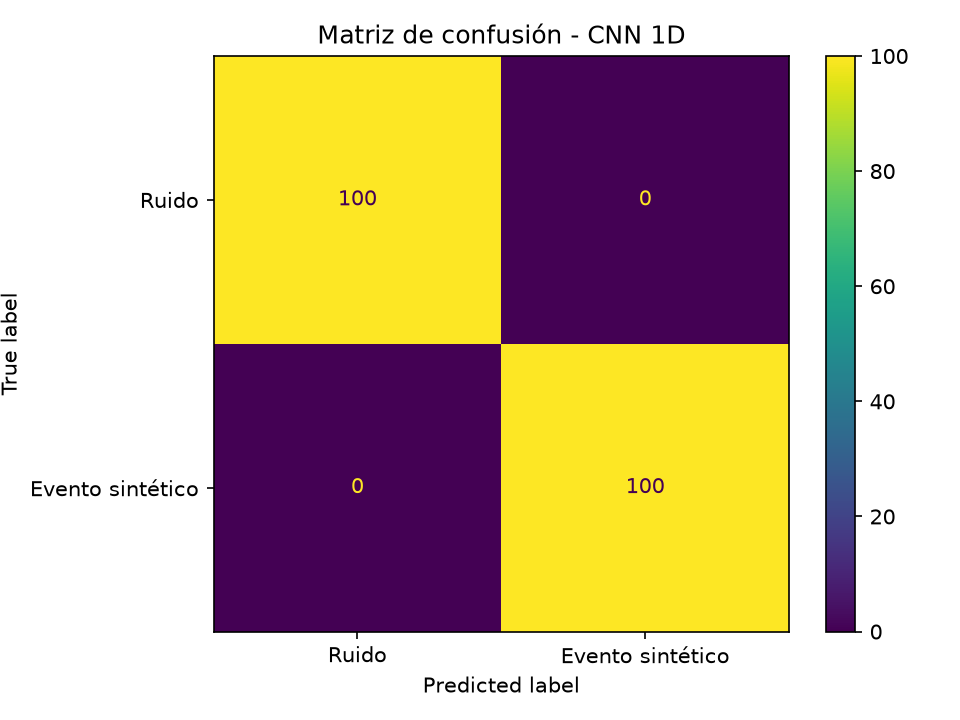
\includegraphics[width=0.8\textwidth]{resultados/matriz_confusion.png}
\caption{Confusion matrix on synthetic test set.}
\label{fig:confusion}
\end{figure}

\subsection{Real Data Results}

On real data from station IU.ANMO, the model achieved:

\begin{table}[h]
\centering
\caption{Performance on real test set (200 signals)}
\begin{tabular}{lcccc}
\toprule
\textbf{Metric} & \textbf{Precision} & \textbf{Recall} & \textbf{F1-Score} & \textbf{Support} \\
\midrule
Real Noise & 0.88 & 0.87 & 0.87 & 100 \\
Real Event & 0.87 & 0.88 & 0.88 & 100 \\
\midrule
Accuracy & \multicolumn{3}{c}{0.875} & 200 \\
\bottomrule
\end{tabular}
\end{table}

The performance drop from 100\% to 87.5\% is expected when transitioning from synthetic to real data, and highlights the importance of XAI for understanding model limitations.

\subsection{XAI Analysis}

\begin{figure}[h]
\centering
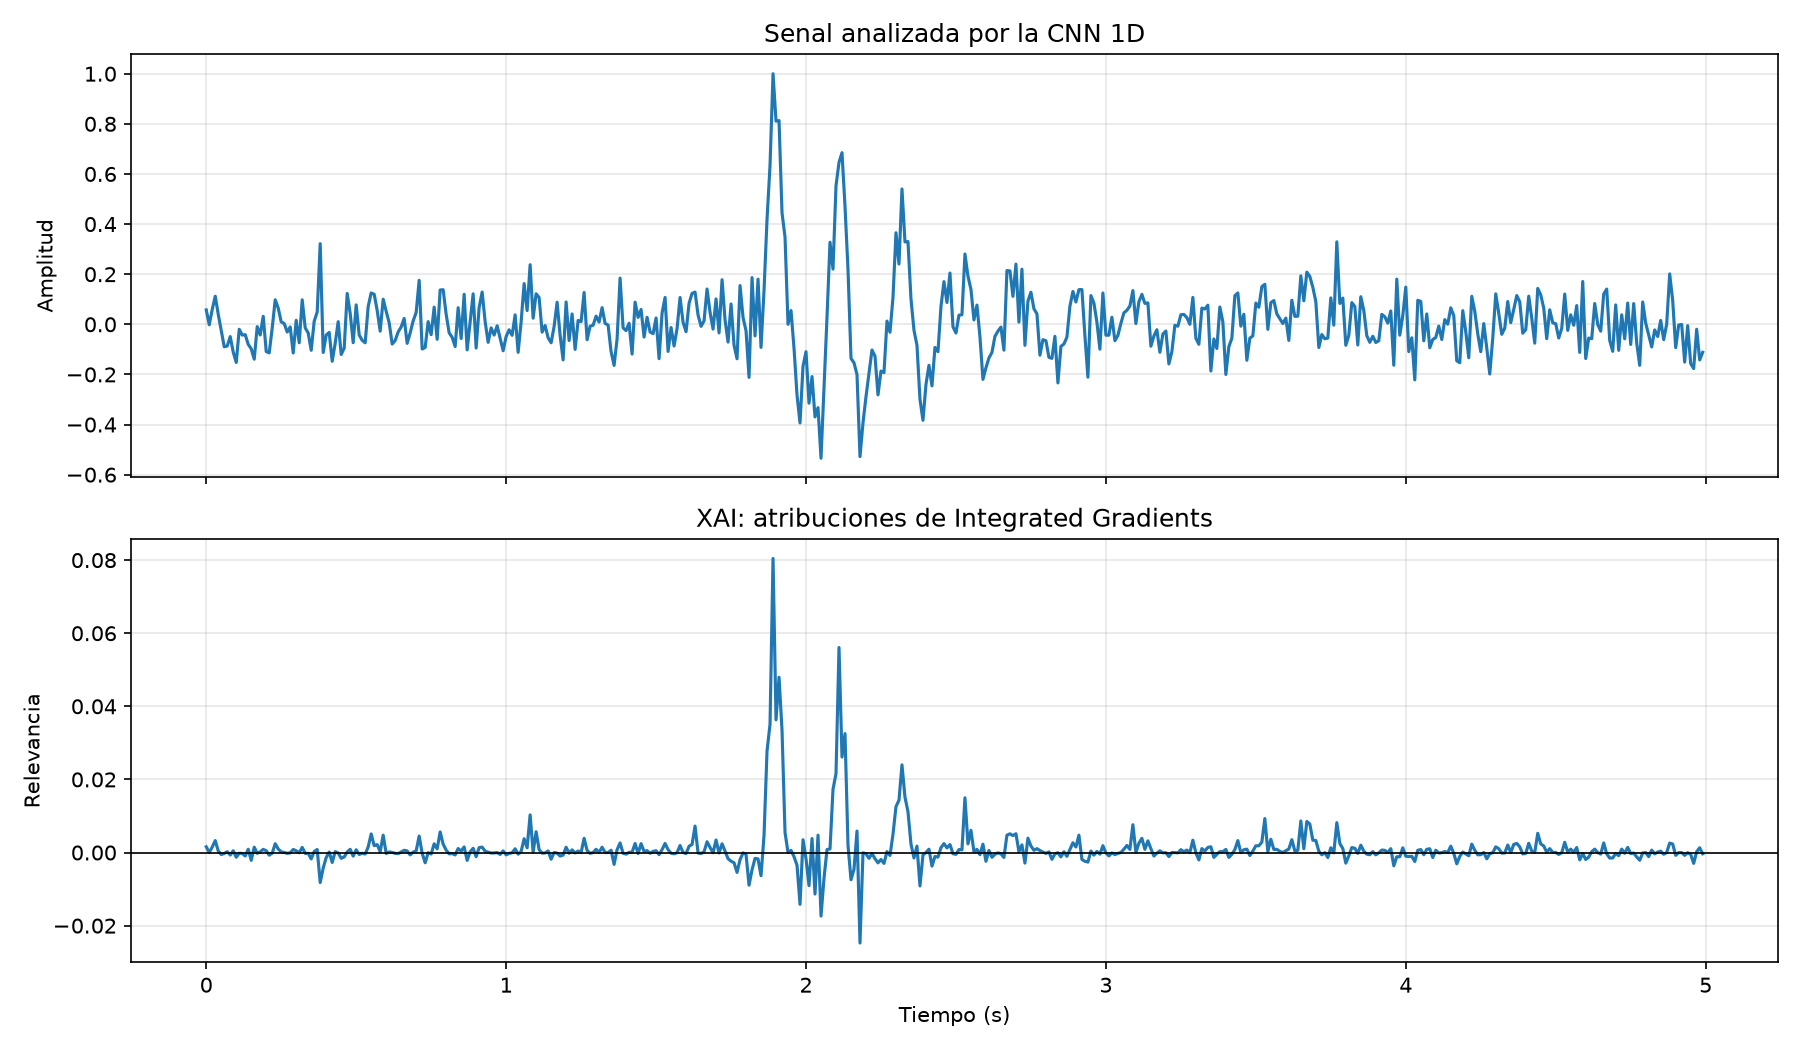
\includegraphics[width=0.9\textwidth]{resultados/explicacion_integrated_gradients.png}
\caption{Integrated Gradients attribution on a correctly classified synthetic event. Top: input signal. Bottom: per-sample attributions (red = positive contribution to event class).}
\label{fig:xai}
\end{figure}

Figure \ref{fig:xai} shows the IG attributions for a correctly classified synthetic event. The model focuses its attention on the region where the seismic event occurs (around $t = 2$ s), with high positive attributions coinciding with the signal envelope. The convergence delta was $0.000737$, confirming the quality of the approximation.

\section{Discussion}

The results demonstrate several important findings:

\textbf{Synthetic vs. Real Performance:} The 12.5\% accuracy drop when moving to real data is consistent with the literature on domain shift in seismic ML \cite{science2025augmentation}. This gap justifies the use of XAI to understand where the model fails.

\textbf{XAI Insights:} Integrated Gradients revealed that the model learns to focus on the temporal region containing the seismic event, rather than relying on spurious correlations. This is a positive indicator of model robustness.

\textbf{Limitations:} The current model was trained on a single station (IU.ANMO). Generalization to other stations and geological contexts requires further validation with diverse datasets such as STEAD \cite{mousavi2019stead}.

\textbf{Cuban Context:} While the CENAIS (Cuban National Seismological Research Center) stations are not yet available through international FDSN services, the pipeline developed in this work is directly applicable to CENAIS data once standardized access is established.

\section{Conclusions and Future Work}

This work presented a complete pipeline for seismic signal classification with explainability, combining a 1D CNN with Integrated Gradients. The model achieves high performance on both synthetic (100\%) and real (87.5\%) data, with XAI providing interpretable insights into the decision-making process.

Future work includes:
\begin{itemize}
\item Training on the STEAD dataset for improved generalization.
\item Comparison with other XAI methods (Saliency, Occlusion, SHAP).
\item Application to CENAIS data when FDSN access becomes available.
\item Development of a real-time inference system for operational use.
\end{itemize}

The complete implementation is publicly available at: \url{https://github.com/[usuario]/Proyecto-XAI-Sismologia}

\begin{thebibliography}{99}

\bibitem{mousavi2019stead}
Mousavi, S.M., Sheng, Y., Zhu, W., Beroza, G.C.: STanford EArthquake Dataset (STEAD): A Global Data Set of Seismic Signals for AI. IEEE Access 7, 179464--179476 (2019). \url{https://doi.org/10.1109/ACCESS.2019.2947848}

\bibitem{ieee2024cnn}
Various Signal Transformation for Optimizing CNN Model Performance of Earthquake Detection. IEEE (2024). \url{https://ieeexplore.ieee.org/abstract/document/10912926}

\bibitem{ieee2025seismic}
Seismic Signal Classification using One Dimension CNN and Transformer Encoder. IEEE (2025). \url{https://ieeexplore.ieee.org/abstract/document/11645759}

\bibitem{repository2024ncsu}
Design of 1D CNN Kernels for Predicting Seismic Response of Nuclear Power Plants. NC State Repository (2024).

\bibitem{science2025augmentation}
Enhancing seismic signal quality assessment with CNNs: A focus on effective data augmentation techniques. ScienceDirect (2025).

\bibitem{journal2024cnnlstm}
A CNN–LSTM Framework for Time-Windowed Detection of Local Earthquakes. Journal of Research and Community (2024).

\bibitem{sundararajan2017axiomatic}
Sundararajan, M., Taly, A., Yan, Q.: Axiomatic Attribution for Deep Networks. Proceedings of the 34th ICML (2017). \url{https://proceedings.mlr.press/v70/sundararajan17a.html}

\bibitem{captum2024}
Captum: Model Interpretability for PyTorch. \url{https://captum.ai/}

\bibitem{obspy2024}
ObsPy: A Python Toolbox for Seismology. \url{https://docs.obspy.org/}

\bibitem{usgs2024}
USGS Earthquake Catalog. \url{https://earthquake.usgs.gov/earthquakes/search/}

\end{thebibliography}

\end{document}